\chapter{Blow up}
\epigraph[author={Michelangelo Antonioni},source={Blow Up}]{Nothing like a little disaster for sorting things out.}
\begin{center}
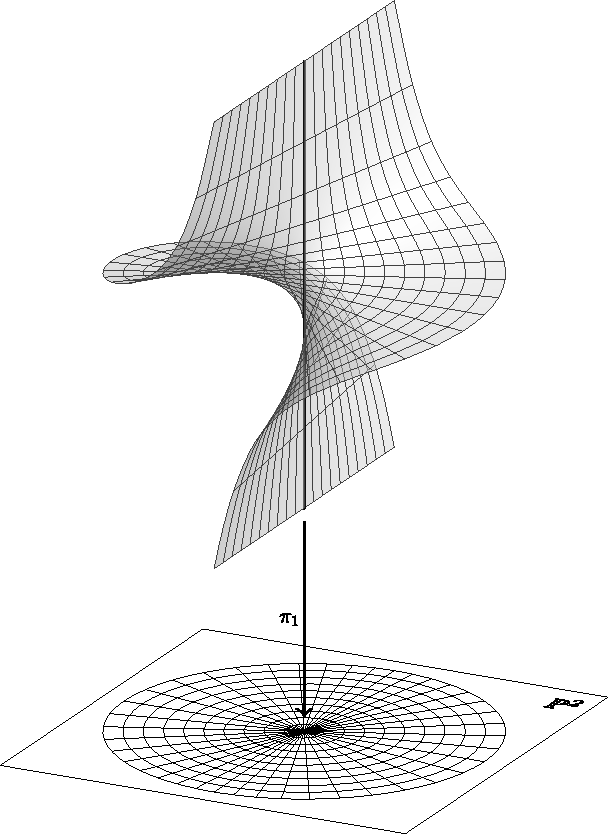
\includegraphics[width=6cm]{blow-up-Staats}
\end{center}

\section{Blowing up curves}
\begin{example}
Take the plane curve \(C=(0=x^2+x^3-y^2)\):
\inputinexample{cubic-curve-1}
The origin is a singular point.
Consider new variables \(X=x,Y=y/x\), which we can write as \(x=X,y=XY\).
In these variables, the same curve is 
\begin{align*}
0
&=
X^2+X^3-(XY)^2,
\\
&=
X^2(1+X-Y^2).
\end{align*}
The curve was an irreducible cubic, but is now a product of a line \(X=0\), appearing twice, and a conic \(1+X=Y^2\).
\end{example}
This is surprising: an irreducible curve reducing, and a cubic which is \emph{not} a union of a line a conic, becomes just that.
Part of the explanation is that the change of variables is not defined along the line \(x=0\), so it is a badly behaved change of variables.
But we can map \((X,Y)\mapsto(x,y)=(X,XY)\) everywhere.
When we do, the \emph{exceptional line}\define{exceptional line} \((X=0)\) (i.e. every point \((X,Y)\) with \(X=0\)) gets mapped to the origin. 
So the map is many to one.
Away from the exceptional line, the map is bijective, but only maps to points \((x,y)\) with \(x\ne 0\).
So the image of the map is the \((x,y)\)-plane, sliced along the line \((x=0)\), but then with the origin glued back in.

Take any plane algebraic curve \(C=(0=p(x,y))\), with singularity at the origin.
Expand out in homogeneous polynomials by degree:
\[
p(x,y)=p_d(x,y)+p_{d+1}(x,y)+\dots+p_n(x,y),
\]
Change variables linearly if needed so that the vertical axis \((x=0)\) is not a tangent line, i.e. \(p_d(0,y)\) is not the zero polynomial.
Plug in the same \((x,y)=(X,XY)\) variables to get
\begin{align*}
p(X,Y)
&=
X^dp_d(1,Y)+X^{d+1}p_{d+1}(1,Y)+\dots+X^np_n(1,Y),
\\
&+
X^d(p_d(1,Y)+Xp_{d+1}(1,Y)+\dots+X^{n-d}p_n(1,Y)).
\end{align*}
So the curve \(C\) splits into two curves: the exceptional line \((X=0)\), which arises with multiplicity \(d\), and the curve
\[
C'=(0=p_d(1,Y)+Xp_{d+1}(1,Y)+\dots+X^{n-d}p_n(1,Y)),
\]
a curve of degree \(n-d\), the \emph{proper transform}\define{proper transform} of \(C\).
The curve \(C\) when written in these \((X,Y)\) variables as above is the \emph{total transform} of \(C\), i.e. just the proper transform together with the multiplicity \(d\) copy of the exceptional line.

\section{Three dimensional pictures}
Take a plane algebraic curve \(C=(0=p(x,y))\) through the origin.
Draw the ``cylinder'' \(X\) consisting of points \((x,y,z)\) in three dimensions with \(0=p(x,y)\).
Intersect the cylinder with the ``saddle surface'' \(S\) consisting of points \((x,y,z)\) with \(y=xz\).
The intersection curve \(\tilde{C}\defeq X\cap S\) consists of points \(0=p(x,y)\) and \(y=xz\).
These equations together force \(0=p(x,xz)\).
So the intersection curve projects to the \((x,z)\)-plane to become two curves: the proper transform and the exceptional line.
We always find the line \((x=y=0)\) lying in the intersection curve; this is the exceptional line in this picture.

Draw the original curve \(C\) on a flat plane, i.e. with constant \(z\).
In dark blue, draw the ``cylinder'' \(X\) connecting \(C\) with  that intersection curve \(\tilde{C}=X\cap S\), but we don't draw \(S\) (just to avoid clutter).
The curve along the top is \(\tilde{C}\), and on the bottom is \(C\). 
The proper transform \(C'\) is the projection of \(\tilde{C}\) to the \((x,z)\)-plane, i.e. we project \(C'\) onto a flat wall to the left of the picture; the flat wall is a plane of constant \(y\).
\begin{center}
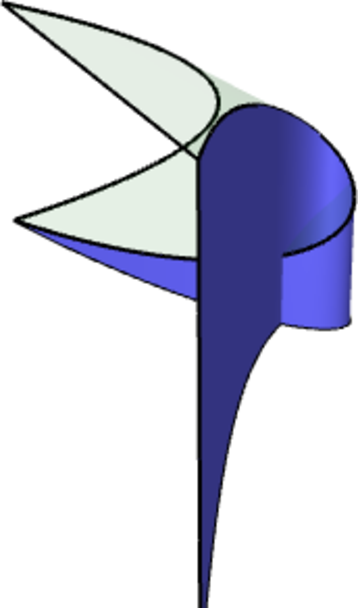
\includegraphics[width=4cm]{blow-up-nodal-cubic}
\end{center}
In sage, you can rotate the picture with your mouse; try
\begin{verbatim}
x(t)=t^2-1
y(t)=t*(t^2-1)
z(t)=t
u,v=var('u,v')
cylindr=parametric_plot3d(
    (x(u), y(u), v*z(u)+(1-v)*(-2)), 
    (u,-2,2), 
    (v,0,1),
    boundary_style={"color": "black", 
                    "thickness": 2,
                    "plot_points":400},
    frame=False,
    plot_points=[300,300])
other_cylindr=parametric_plot3d(
    (x(u), v*y(u)+(1-v)*(-6), z(u)), 
    (u,-2,2), 
    (v,0,1),
    color="green",
    opacity=.1,
    boundary_style={"color": "black", 
                    "thickness": 2,
                    "plot_points":400},
    frame=False,
    plot_points=[300,300])
show(cylindr+other_cylindr)
\end{verbatim}

\section{Blowing up singularities}
Let us reconsider the story algebraically.
In some algebraic extension, we factor \(p_d(x,y)\), say into
\[
p_d(x,y)=(y-m_1x)(y-m_2x)\dots(y-m_dx).
\]
There is no \(x\) factor, because we supposed that the vertical axis is not tangent.
The equation of \(C\) becomes in \(X,Y\):
\begin{align*}
0&=
p_d(X,XY)+\dots,
\\
&=
(XY-m_1X)(XY-m_2X)\dots(XY-m_dX)+\dots,
\\
&=
X^d(Y-m_1)(Y-m_2)\dots(Y-m_d)+\dots.
\end{align*}
So the \(Y\) variable keeps track of the slopes of the tangent lines.
Indeed since \(Y=y/x\), we can think of \(Y\) as a slope.
The proper transform has equation
\[
0=(Y-m_1)(Y-m_2)\dots(Y-m_d)+Xp_{d+1}(1,Y)+\dots+X^{n-d}p_n(1,Y)
\]
so at \(X=0\), the roots of the proper transform are the slopes of the tangent lines.
\begin{example}
Again take the plane curve \(C=(0=x^2+x^3-y^2)\):
\inputinexample{cubic-curve-1}
The proper transform is \(C'=(1-Y^2+X)\), so has \(X=0\) term \(1-Y^2=(1-Y)(1+Y)\), the two slopes of the two tangent lines are \(Y=\pm 1\).
\end{example}
Each root \(Y=m_i\) occurs as the intersection of the proper transform \(C'\) with the line \(X=0\), i.e. the exceptional line, with multiplicity equal to the number of factors of \(y-m_ix\) in the lowest degree terms \(p_d(x,y)\).
By theorem~\vref{theorem:multiplicity.submultiplicative}, that intersection number is no less than the multiplicity of \(C'\) at each intersection point \((X,Y)=(0,m_i)\).

The intersection number of each tangent line \(\ell=(y=m_ix)\) with \(C\) is, from theorem~\vref{theorem:tangent.intersection}, given by plugging in \(y=m_ix\) to the equation of \(C\), i.e. into \(p(x,y)\), and counting the degree of \(p(x,m_ix)\) as a function of \(x\).

The multiplicity of \(C\) at the origin is the sum of multiplicities of tangent lines.
So the multiplicities of \(C'\) along the exceptional line add up to at most the multiplicity of \(C\) at the origin, with equality just when there is a unique tangent line to \(C\) (in any extension field), so \(p_d\) is a power of a single linear factor.
\begin{example}
The cuspidal cube \(C=(y^2=x^3)\)
\inputinexample{cubic-curve-cuspidal}
has proper transform \(C'=(Y^2-X)\), which intersects the exceptional line \((X=0)\) as \(Y^2=0\), i.e. with multiplicity \(2\).
\includegraphicsinexample[width=7cm]{blow-up-cuspidal-cubic}
\end{example}

\section{Blowing up the plane}
The pictures help, especially if you get sage to draw them in three dimensions.
But there is still the uncomfortable feeling that (i) we had to arrange that the vertical axis is not a tangent line, which seems artificial and (ii) the story occurs in the affine plane, but the true story should arise in the projective plane.

Rather than thinking of variables \(X=x,Y=y/x\), think that \(Y\) is the slope of the line from the origin to \((x,y)\).
That line is determined by its slope, so \(Y\) parameterizes the lines through the origin by their slopes.
Pick a point, which we can think of as the origin, and draw all of the lines through it.
The \emph{blow up} \(B_{p_0}\) at a point \(p_0\) of the projective plane is the set of all pairs \((p,\ell)\) so that \(p\) is a point of the projective plane, \(\ell\) a projective line on the plane passing through \(p_0\), and \(p\) is also a point of \(\ell\).

If we draw the real projective plane, or more precisely affine coordinates, and draw each line \(\ell\) through the origin of affine coordinates, so that we lift it up higher if it has higher slope, we get a picture (due to Charles Staats III) at the beginning of this chapter.
The blow up is the surface drawn twisting around above the plane.

Let's become more closely acquanted with the picture.
Each point \(q\) of the blow up drops straight down to a point \(p\) of the plane.
If \(p\) is not the origin, then the line \(\ell\) is the line through the origin and \(p\), and we can recover \(q\) as the unique point of the blow up surface lying directly above \(p\).
If \(p\) is the origin, then the point \(q\) lies on the \emph{exceptional line}, the line drawn directly above the origin.
But then the line \(\ell\) is the unique line in the plane so that the line on the blow up which projects down to \(\ell\) passes through \(q\).

Algebraically: take the projective plane \(P\) and its dual plane \(P^*\).
We can write points of \(P\) as \(p=[x_0,x_1,x_2]\) and points of \(P^*\) as 
\(\ell=[a_0,a_1,a_2]\), corresponding to the line \(0=a_0x_0+a_1x_1+a_2x_2\) in \(P\).
The line \(\ell\) goes through the origin \(p_0=[0,0,1]\) of the affine plane just when \(a_2=0\).
The line \(\ell\) also goes through the point \(p\) just when \(0=a_0x_0+a_1x_1\).
So the blow up surface \(B_{p_0}\) is the set of all pairs 
\[
(p,\ell)=([x_0,x_1,x_2],[a_0,a_1,0])\in P \times P^*
\] 
so that \(a_0x_0+a_1x_1=0\).
So the blow surface is the intersection of the two three dimensional varieties: the \emph{incidence variety} \((a_0x_0+a_1x_1+a_2x_2=0)\subset P \times P^*\), consisting of pointed lines, and the variety \(P\times p_0^*\).

The \emph{exceptional divisor} \(E_{p_0}\) is the subset of \(B_{p_0}\) consisting of points \((p_0,\ell)\) where \(\ell\) is a line through \(p_0\).
The set of these lines \(\ell\) form a projective line inside the projective plane \(P^*\).

Take an algebraic curve \(C\) in the projective plane \(P\) and a point \(p_0\) of \(P\).
The points of \(B_{p_0}\) away from the exceptional divisor are points \((p,\ell)\) where \(p\ne p_0\) and \(\ell\) is the line \(p_0 p\).
Each such point is uniquely identified with the point \(p\).
The points of \(B_{p_0}\) lying over the points of \(C\), and not over the point \(p_0\), are precisely those of the form \((p,\ell)\) where \(p\) is a point of \(C\) and \(\ell=p_0 p\), so identified with the points \(p\) of \(C\). 
The closure of that set of points is the \emph{strict transform} of \(C\).
